\chapter{Background}

\section{Electromagnetic Fields}
The electromagnetic fields are a collection of closely linked fields.
These fields govern the electric and magnetic interactions of charged
particles and domains. These fields can be seen in table \ref{tab:fields}

\begin{center}
    \begin{tabular}{c c c}
        \label{tab:fields}
        Field    & SI unit         & Description              \\
        \hline
        $\vb{H}$ & $1\, Am^{-1} $  & Magnetic Field           \\
        $\vb{E}$ & $1\, Vm^{-1} $  & Electric Field           \\
        $\vb{B}$ & $1\, Vsm^{-2} $ & Magnetic Flux Density    \\
        $\vb{D}$ & $1\, Asm^{-2} $ & Electric Flux Density    \\
        $\vb{J}$ & $1\, Am^{-2} $  & Electric Current Density \\
        $\rho$   & $1\, Asm^{-3} $ & Electric Charge Density
    \end{tabular}
\end{center}
These fields are described by Maxwells Equations.
In differential form for the stationary case, these are as follows:

\begin{align}
    \nabla \times \vb{H} & = \vb{J} + \frac{\partial}{\partial t}\vb{D}
    \label{eq:maxwell1}                                                 \\
    \nabla \times \vb{E} & = -\frac{\partial}{\partial t}\vb{B}
    \label{eq:maxwell2}                                                 \\
    \nabla \cdot \vb{B}  & = \vb{0}
    \label{eq:maxwell3}                                                 \\
    \nabla \cdot \vb{D}  & = \rho
    \label{eq:maxwell4}
\end{align}
Since we're dealing with measurement of magnetic fields in this thesis,
equations \ref{eq:maxwell1} and \ref{eq:maxwell3} will naturally be of
the most interest. In simple cases, the $\vb{H}, \vb{D}, \vb{E}$ and
$\vb{B}$ field obey the easy relations
\begin{align}
    \vb{B} & = \mu \vb{H}
    \label{eq:BHmap}           \\
    \vb{D} & = \epsilon \vb{E}
\end{align}
where $\mu$ is the \emph{magnetic permeability} and $U$ is the
\emph{electric permittivity} in the domain of interest.
Formally, simple cases are where the fields are located in a medium that is
linear, homogenous across its domain, invariant depending on direction, and
stationary. Since the magnetic measurements are made inside the empty aperture
of the magnet, the domain is only made up of air. Thus, equation \ref{eq:BHmap}
holds, and the magnetic permeability is the one of free space, that is
$\mu = \mu_0 = 4\pi \times 10^{-7} Hm^{-1}$. \cite[Ch.4.1-4.4]{russenschuck2011field}


\subsection{Magnetic Flux and Induction}
Magnetic flux $\Phi$ is the surface integral of the $\vb{B}$ field
along the normal vector to the surface.
Mathematically, it is defined as:
\begin{equation}
    \Phi(\area) = \iint\limits_{\area} \vb{B} \cdot \nvec\, d\area
\end{equation}
where $\area$ is the surface, and $\nvec$ is the normal vector to the surface.
We then have the following governing laws of electromagnetism for objects at rest:
\begin{align}
    U(\partial\area)      & = -\frac{d}{dt}\Phi(\area)
    \label{eq:faraday}                                 \\
    \Phi(\partial\Volume) & = 0
    \label{eq:fluxcons}
\end{align}

\begin{figure}
    \centering
    \begin{subfigure}[b]{0.4\textwidth}
        \centering
        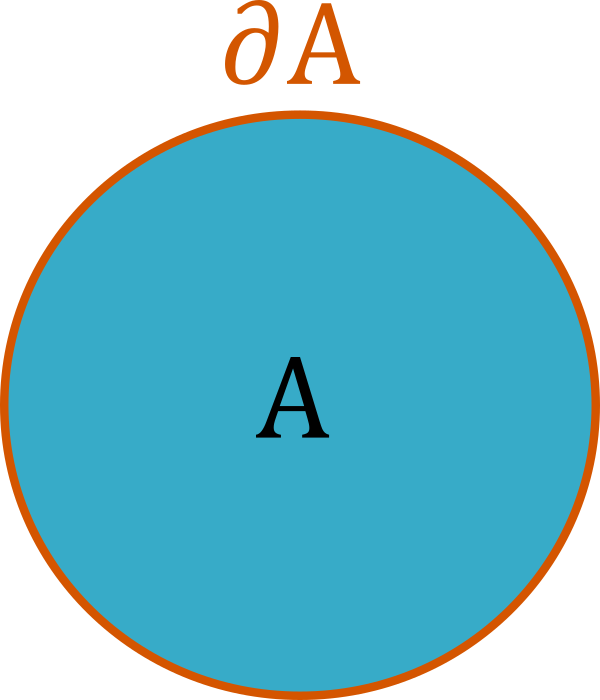
\includegraphics[height=125pt]{figs/partialA}
        \caption{An area $\area$ and its boundary $\partial \area$. }
        \label{fig:partialA}
    \end{subfigure}
    \hfill
    \begin{subfigure}[b]{0.4\textwidth}
        \centering
        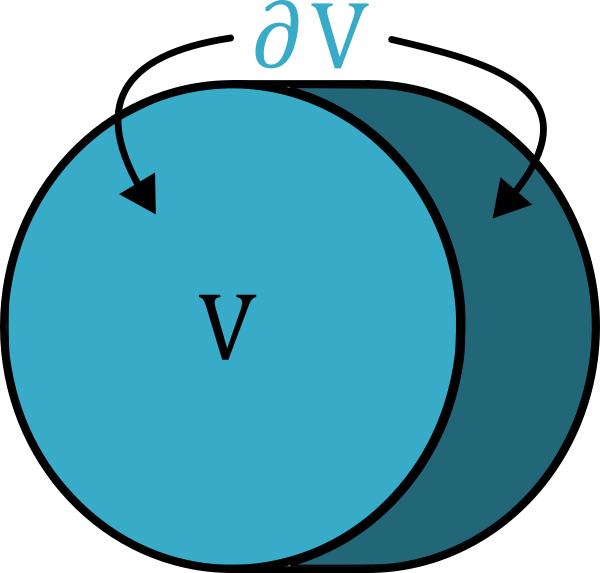
\includegraphics[height=125pt]{figs/partialV}
        \caption{A volume $\Volume$ and its surface boundary $\partial \Volume$.}
        \label{fig:partialV}
    \end{subfigure}
\end{figure}
Equation \ref{eq:faraday}, also called faradays law, describes the voltage\
$\epsilon$ induced in a length of wire $\partial\area$, enclosing an area
$\area$, when the magnetic flux $\Phi$ is changing with respect to time.
The signs of $U$ and $\Phi$ obey the right hand rule as indicated
in figure \ref{fig:partialA}.

Equation \ref{eq:fluxcons} states that the total amount of flux flowing
through the boundary $\partial\Volume$ of the volume
$\Volume$ must equal 0.\cite[Ch.4.1.1]{russenschuck_field_2011}

\section{Series decompositions of the magnetic field}
The magnetic field can be calculated in some different ways, for instance
directly from Maxwells equations or using Biot-Savarts law:
\begin{equation}
    \vb{B}(\vb{r}) = \frac{\mu_0}{4\pi}\int\limits_\Volume
    \frac{\vb{J}(\vb{r'})\times (\vb{r} - \vb{r'})}
    {|\vb{r} - \vb{r'}|^3} d\Volume
\end{equation}
where $\vb{B}(\vb{r})$ is the $\vb{B}$ field at coordinate $\vb{r}$ and
$\vb{J}(\vb{r'})$ is the current distribution at coordinate $\vb{r'}$.
\cite[Ch.5.4]{russenschuck2011field}
Except for very simple geometries, the magnetic field is rarely
expressible using elementary functions. A common method is then
to express it using fourier series solutions inside a specified domain.
\cite[Ch.6]{russenschuck2011field}

Inside the aperture of a magnet, the domain is free of currents and made
up of air or vacuum. The current powering the magnet is constant,
meaning we have a constant electric field. Equation \ref{eq:maxwell1}
can then be rewritten as follows:
\begin{align}
    \begin{split}
        \nabla \times \vb{H} &= \mu_0\nabla \times \vb{B}\\
        \mu_0\nabla \times \vb{B}
        &=\vb{J} + \frac{\partial}{\partial t}\vb{D}
        \Bigg\vert_{\substack{\vb{J}=\vb{0} \\
                \frac{\partial}{\partial t}\vb{D}=\vb{0}}} \\
        &= \vb{0}
    \end{split}
\end{align}
This, along with equation \ref{eq:maxwell3} means that there
exists a magnetic scalar potential $\Psi(\vb{r})$ of $\vb{B}$ that satisfies
Laplace's equation
\begin{equation}
    \nabla^2\Psi = \frac{\partial^2 \Psi}{\partial x^2}
    + \frac{\partial^2 \Psi}{\partial y^2}
    + \frac{\partial^2 \Psi}{\partial z^2} = 0
    \label{eq:laplacian_zero}
\end{equation}
inside the domain, where the $\vb{B}$ field components are
\begin{equation}
    B_x = \frac{\partial \Psi}{\partial x}, \,
    B_y = \frac{\partial \Psi}{\partial y}, \,
    B_z = \frac{\partial \Psi}{\partial z}
\end{equation}
\subsection{Cylindrical Coordinates}
Since the aperture of our magnet is cylindrical, working in cylindrical
coordinates $(r, \varphi, z)$ is a natural choice. They are related to the cartesian
system $(x, y, z)$ through the relations:

\begin{align}
    \begin{split}
        x &= r\cos \varphi \\
        y &= r\sin \varphi \\
        z &= z
    \end{split}
\end{align}

\begin{wrapfigure}{r}{0.5\textwidth}
    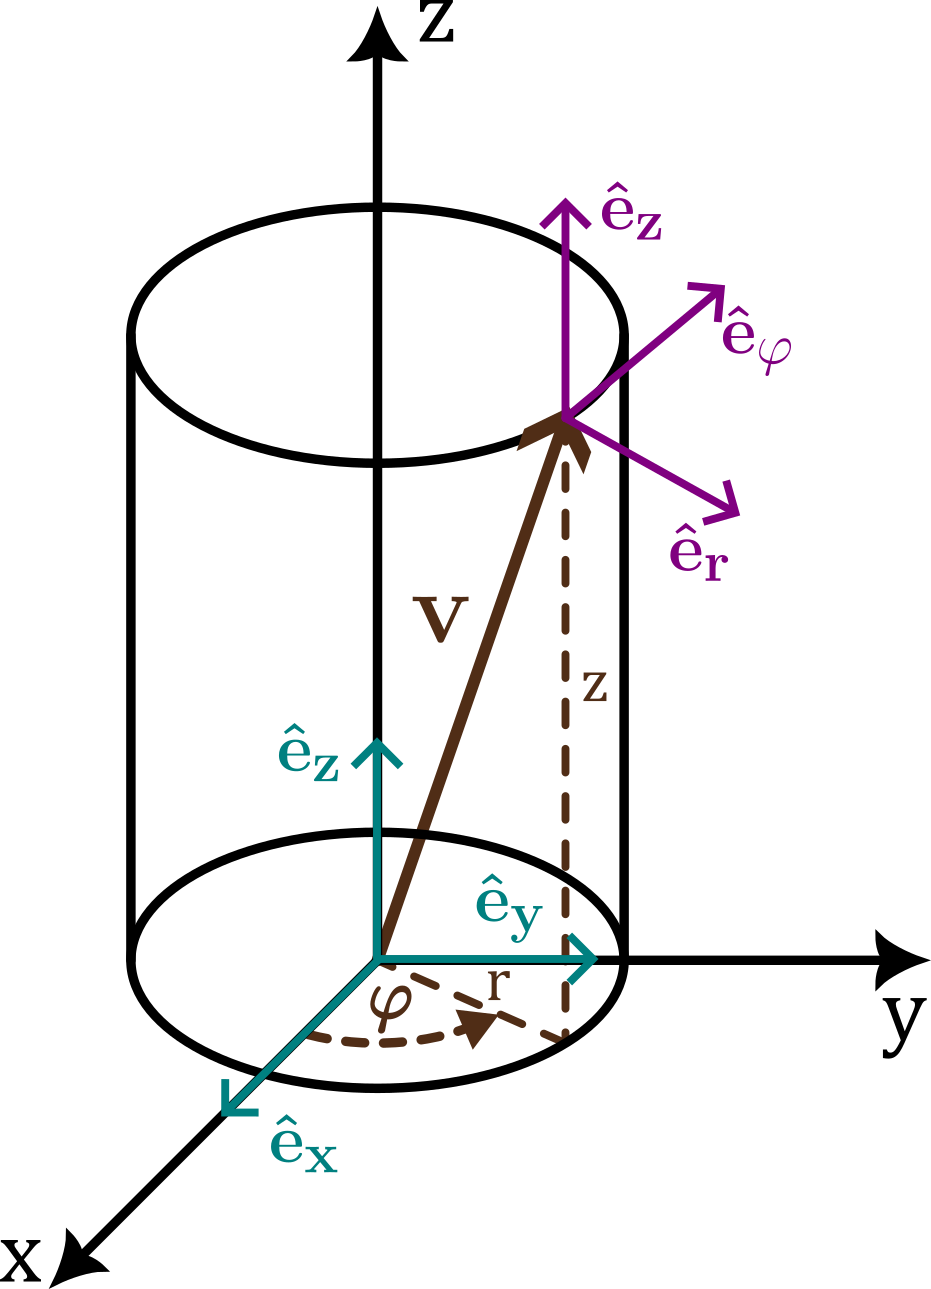
\includegraphics[width=0.5\textwidth]{figs/cylcoords}
    \caption{Cylindrical coordinates and their relationship to cartesian coordinates.}
    \label{fig:cylcoords}
\end{wrapfigure}

A vector $\vb{v}$ is defined by its distance $r$ from the origin, its
angle $\varphi$ from the $x$-axis, and its offset in $z$ as
$\vb{v}(r, \varphi, z)  = (r\cos \varphi, r\sin \varphi, z)$.
Where in cartesian coordinates we have
the basis vectors $\ex, \ey, \ez$
along the x, y and z axis, in cylindrical coordinates we have
$\er, \ephi, \ez$ as illustrated in
figure \ref{fig:cylcoords}. Note that $\er$ and $\ephi$
change direction depending on the current value of $\varphi$.

\subsubsection{Scaling Factors}
In cylindrical coordinates, scaling factors are needed for
common differential operators. For a scalar field $\Psi(r, \varphi, z)$
the gradient is defined as
\begin{equation}
    \nabla \Psi = \frac{\partial \Psi}{\partial r} \er +
    \frac{1}{r} \frac{\partial \Psi}{\partial \varphi} \ephi +
    \frac{\partial \Psi}{\partial z} \ez
    \label{eq:cylgrad}
\end{equation}

The divergence of a vector field $\vb{V}(r, \varphi, z)$ is
\begin{equation}
    \nabla \cdot \vb{V} = \frac{1}{r} \frac{\partial}{\partial r} (rV_r)
    + \frac{1}{r} \frac{\partial V_\varphi}{\partial \varphi}
    + \frac{\partial V_z}{\partial z}
    \label{eq:cyldiv}
\end{equation}
which gives the laplacian $\nabla^2 \Psi = \nabla \cdot \nabla \Psi (r, \varphi, z)$
\begin{equation}
    \nabla^2 \Psi =
    \frac{1}{r} \frac{\partial}{\partial r} \left(r\frac{\partial \Psi}{\partial}\right)
    + \frac{1}{r^2} \frac{\partial^2 \Psi}{\partial \varphi^2}
    + \frac{\partial^2 \Psi}{\partial z^2}
    \label{eq:cyl_laplacian}
\end{equation}
\cite[Ch.3.13]{russenschuck2011field}
\subsubsection{The Laplace Equation in Cylindrical Coordinates}
One way to solve the laplacian is to use separation of variables
technique to find the set of potential solutions, and from that
set choose the ones that make sense for our problem.

Firstly, we make the ansatz that the solutions can be written in
the form
\begin{equation}
    \Psi(r, \varphi, z) = R(r)\varPhi(\varphi)Z(z)
    \label{eq:psi_ansatz}
\end{equation}

Insertion of equation \ref{eq:psi_ansatz} into \ref{eq:cyl_laplacian}
then gives us
\begin{equation}
    \nabla^2 \Psi = \frac{1}{rR} \frac{d}{dr} \left(\frac{dR}{dr} \right)
    + \frac{1}{r^2 \varPhi} \frac{d^2 \varPhi}{d\varphi^2}
    + \frac{1}{Z} \frac{d^2 Z}{dz^2}
    \label{eq:sepLaplacian}
\end{equation}

We know from equation \ref{eq:laplacian_zero} that this is equal to zero,
and can therefore rewrite as
\begin{equation}
    -\frac{1}{\varPhi} \frac{d^2 \varPhi}{d\varphi^2} =
    \frac{r}{R} \frac{d}{dr} \left(\frac{dR}{dr} \right)
    + \frac{r^2}{Z} \frac{d^2 Z}{dz^2}
\end{equation}
Here, a contradiction emerges. A change in $\varphi$ can only
introduce a change in the left hand side of this equation. Likewise,
this equality must still hold for a change in $r$ or $z$. These
conditions only hold under the assumption that both sides are constant,
such that
\begin{equation}
    \frac{1}{\varPhi} \frac{d^2 \varPhi}{d\varphi^2} = \alpha_1
\end{equation}
where $\alpha_1$ is constant. Using similar reasoning for $Z(z)$
and then $R(r)$ we can reduce this partial differential equation to
a system of ordinary differential equations.
\begin{align}
    \frac{d^2R}{dr^2} + \frac{1}{r} \frac{dR}{dr} & =
    \left( \frac{\alpha_1}{r^2} + \alpha_2 \right)R
    \label{eq:diffeqR}                                                \\
    \frac{d^2 \varPhi}{d\varphi^2}                & = \alpha_1\varPhi
    \label{eq:diffeqPhi}                                              \\
    \frac{d^2 Z}{dz^2}                            & = \alpha_2 Z
    \label{eq:diffeqZ}
\end{align}

While the differential equations in $\varPhi$ and $Z$ have a well defined
set of solutions using elementary functions like sines, cosines and exponentials,
equation \ref*{eq:diffeqR} is a bit trickier. This equation is known as
the Bessel differential equation, and solving it will require a
set of functions known as the Bessel functions.

\subsection{Bessel Functions}
The Bessel functions are defined as the solutions to equation \ref*{eq:diffeqR}.
They come in several different variants depending on the values of $\alpha_1$ and
$\alpha_2$. They are not expressible using elementary functions and are therefore
often approximated using power series solutions, generating functions
or numeric integration.

The actual calculation of the Bessel functions is outside the scope of this thesis,
more than stating that they are implemented in most popular programming languages.
Still, a short overview of the properties of the most relevant subset of Bessel
functions will aid greatly in finding the solutions to our magnetic scalar potential.

\subsubsection{Bessel Function, First Kind}

The Bessel function of the first kind is a collection of functions that are nonsingular
at the origin. It is often denoted $\Jn{n}(x)$. Figure \ref*{fig:Jnplot} shows
$\Jn{n}(x)$ for $n=0,1,2,3,4$.

\begin{figure}
    \centering
    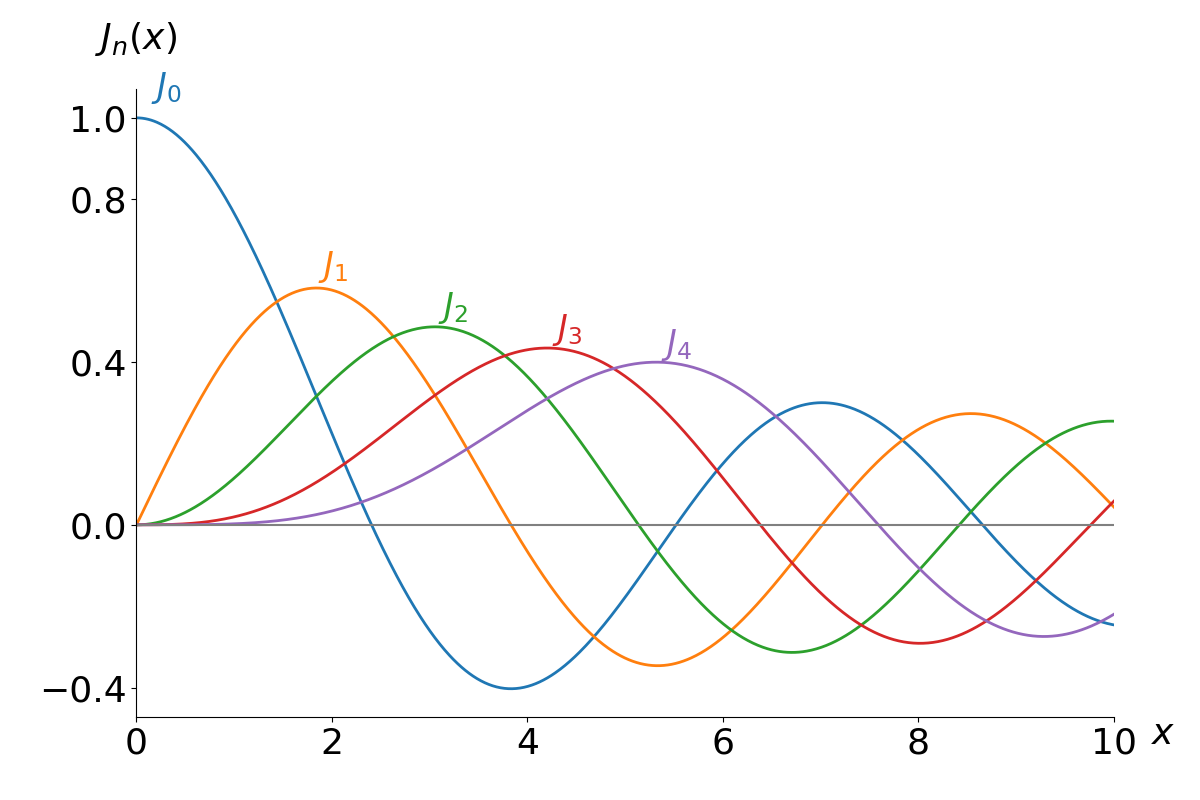
\includegraphics[width=0.8\textwidth]{figs/Jnplot.png}
    \caption{Bessel functions of the first kind, for $n\in[0,4]$.}
    \label{fig:Jnplot}
\end{figure}

For negative $n$ we have
\begin{equation}
    \Jn{-n}(x) = (-1)^n \Jn{n}(x)
\end{equation}

\subsubsection{Modified Bessel Function, First Kind}
For the bessel function of the first kind with imaginary
arguments, the modified Bessel function $\In{n}(x)$ is often used.
It is related to the regular first kind Bessel function
through the equality
\begin{equation}
    \In{n}(x) = j^{-n}\Jn{n}(jx)
\end{equation}

The first five terms of $\In{n}$ can be seen in figure \ref*{fig:Inplot}.

\begin{figure}
    \centering
    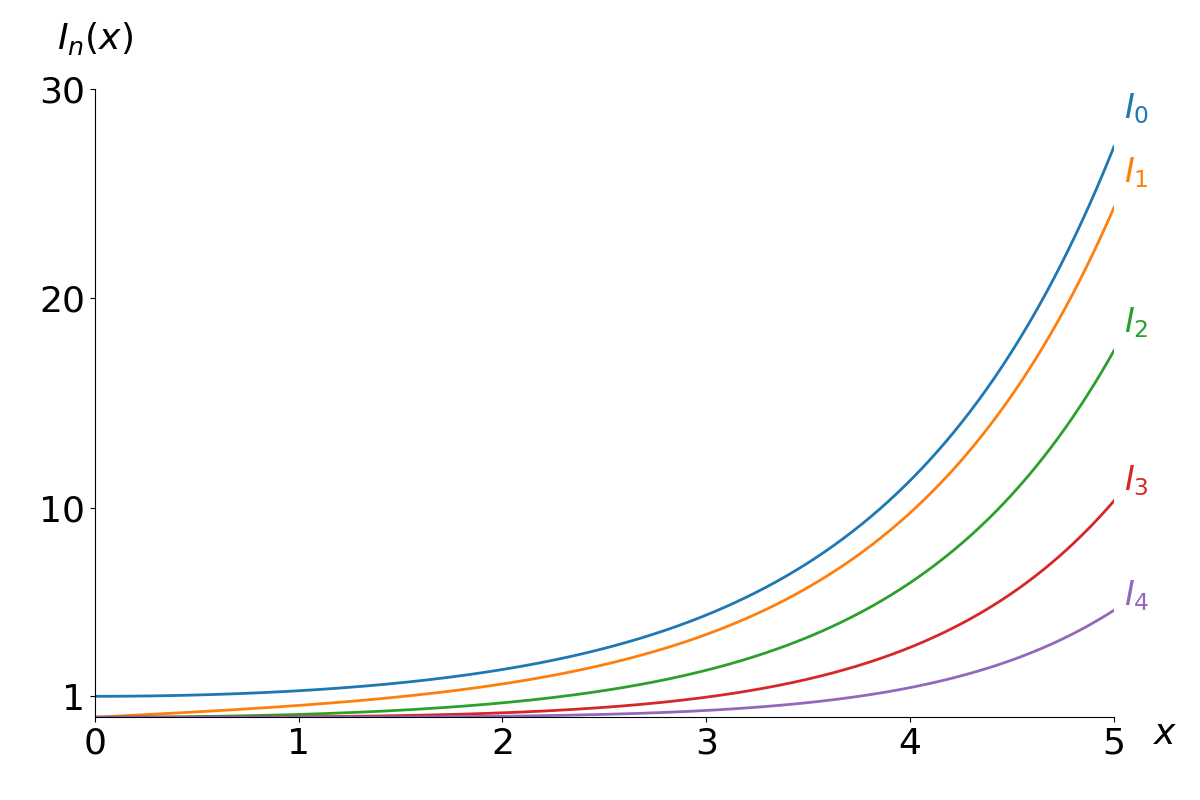
\includegraphics[width=0.8\textwidth]{figs/Inplot.png}
    \caption{Modified Bessel functions of the first kind, for $n\in[0,4]$.}
    \label{fig:Inplot}
\end{figure}

\subsubsection{Bessel Function, Second Kind}
The bessel function of the second kind is a solution to
the bessel differential equation that is singular at the
origin. It can be seen in figure \ref{fig:Ynplot}.

\begin{figure}
    \centering
    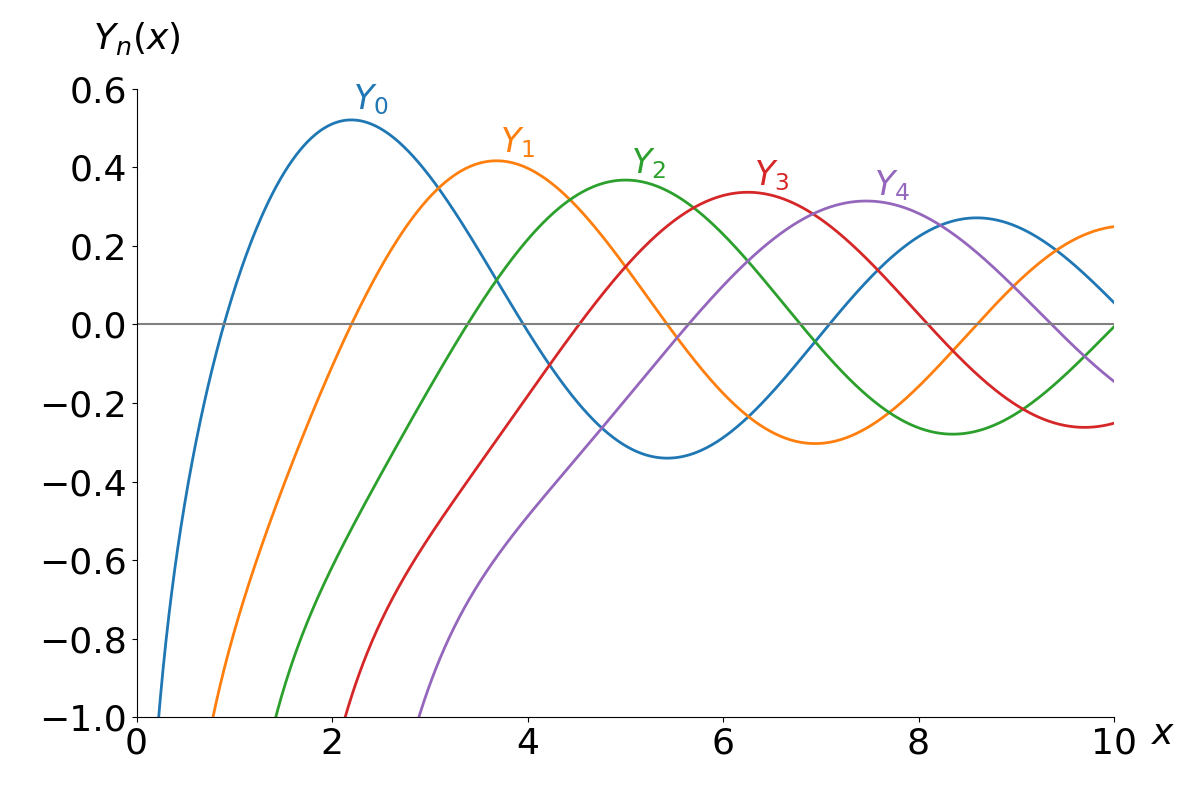
\includegraphics[width=0.8\textwidth]{figs/Ynplot.png}
    \caption{Bessel functions of the second kind, for $n\in[0,4]$.}
    \label{fig:Ynplot}
\end{figure}

\subsection{Bessel-Fourier-Fourier Series}
With

\section{Signal Processing}
\subsection{Filters}
\subsection{Least Squares Fitting}